\paragraph{La classe ObjectFragment}

\begin{minipage}
    {\linewidth}
    \centering
    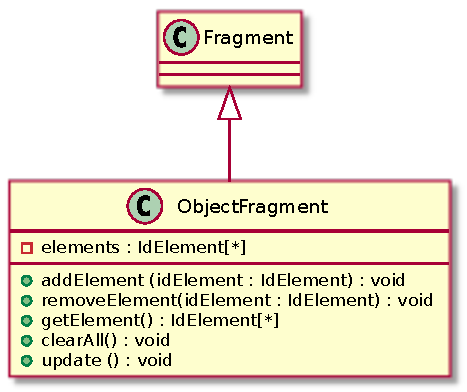
\includegraphics[width=0.80\linewidth]{../schemas/Conception_detaillee/classe_basket.pdf}
    \captionof{figure}{Diagramme de classe de ObjectFragment}
\end{minipage}

\subparagraph{Philosophie de conception \newline} 

\medspace

La classe ObjectFragment est la classe gère le fragment des objets. Elle a aussi pour objectif d'effectuer les  ajouts et soustractions d'éléments. Les opérations étant déjà détaillées dans la conception générale, elles seront uniquement listées.

\subparagraph{Description structurelle \newline}

\medspace

\textbf{Attributs :}

N.A.

\textbf{Services offerts :}

\begin{itemize}
    \item \textbf{elements : IdElement[*]} 
    \item \textbf{addElement (idElement : IdElement)} 
    \item \textbf{removeElement(idElement : IdElement)} 
    \item \textbf{getElements() : IdElement[*]} 
    \item \textbf{clearAll()} 
    \item \textbf{update () : void}


\end{itemize}


\paragraph{La classe BasketAdapter}

\begin{minipage}
    {\linewidth}
    \centering
    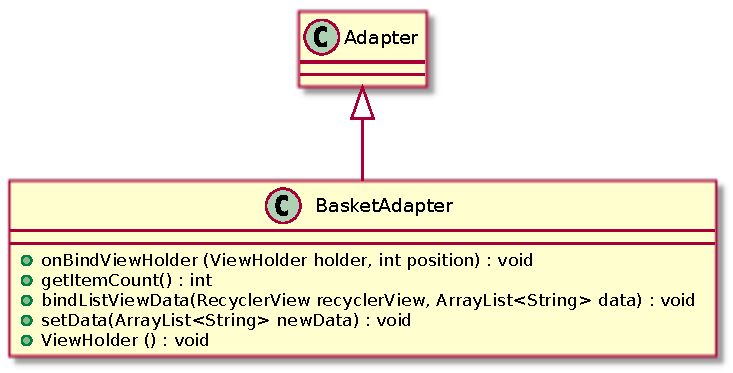
\includegraphics[width=0.80\linewidth]{../schemas/Conception_detaillee/classe_basketAdapter.pdf}
    \captionof{figure}{Diagramme de classe de BasketAdapter}
\end{minipage}

\subparagraph{Philosophie de conception \newline} 

\medspace

La classe BasketAdapter est la classe d'adapter du listView qui gère les items des objets. Elle permet de mettre en forme chaque éléments individuellement et de mettre en forme l'assemblage.

\subparagraph{Description structurelle \newline}

\medspace

\textbf{Attributs :}

N.A.

\textbf{Services offerts :}

\begin{itemize}
    \item \textbf{onBindViewHolder (ViewHolder holder, int position) : void} --- Opération qui permet le binding du ViewHolder. 
    \item \textbf{getItemCount() : int} --- Opération qui permet de retourner le nombre d'items à répartir dans la liste. 
    \item \textbf{bindListViewData(RecyclerView recyclerView, ArrayList<String> data) : void} --- Opération qui permet le binding du listView.
    \item \textbf{setData(ArrayList<String> newData) : void} --- Opération qui permet la mise à jour de la liste.
    \item \textbf{ViewHolder () : void} --- Classe qui permet la création du ViewHolder pour positionner chaque élément individuellement.


\end{itemize}
